\section{課題 3 演習ガイド}
%
%%% CRYPTANALYSIS
%
\subsection{暗号解読 (Cryptoanalysis)}
\begin{frame}[containsverbatim,shrink]
\frametitle{暗号解読}
  \begin{itemize}
\item 暗号をやぶろうとすることを暗号解読 (cryptoanalysis) と呼ぶ
\item 暗号アルゴリズム (\(\cal E\) と \(\cal D\)) は知っているが,鍵を知らないという前提
\item Cipher text only attack: 暗号文だけを得ることができるとして解読 (e.g. 踊る人形)
\item Known plaintext attack: 平文とその暗号文を得ることができるとして解読 (e.g. エニグマで "異常なし")
\item Chosen plaintext attack: 特定の平文を送り,埋め込んだ暗号文を得ることができるとして解読 (e.g. 日本軍のミッドウェイ島攻撃)
  \end{itemize}
\end{frame}
\subsection{課題 3 のシチュエーション}
\begin{frame}[containsverbatim,label=situation,shrink]
\frametitle{課題 3 のシチュエーション}
  \begin{itemize}
\item Alice と Bob が通信しているとして,そこに Eve (eavesdropper) がいるとします
\item 通信の内容を盗み見られないように暗号化して通信します
\item 暗号化の手順は以下の通り
    \begin{enumerate}
\item 送りたい文 (平文 $m$) を暗号化 (encryption) して暗号文 $c$ を作成
\item 暗号文 $c$ を送信
\item 暗号文 $c$ を受信
\item 暗号文 $c$ を復号 (decryption) して平文 $m$ を得る
    \end{enumerate}
\item Eve はこの通信の内容を盗み見て暗号文だけが入手可能で暗号解読を試みる
  \end{itemize}
  \begin{center}
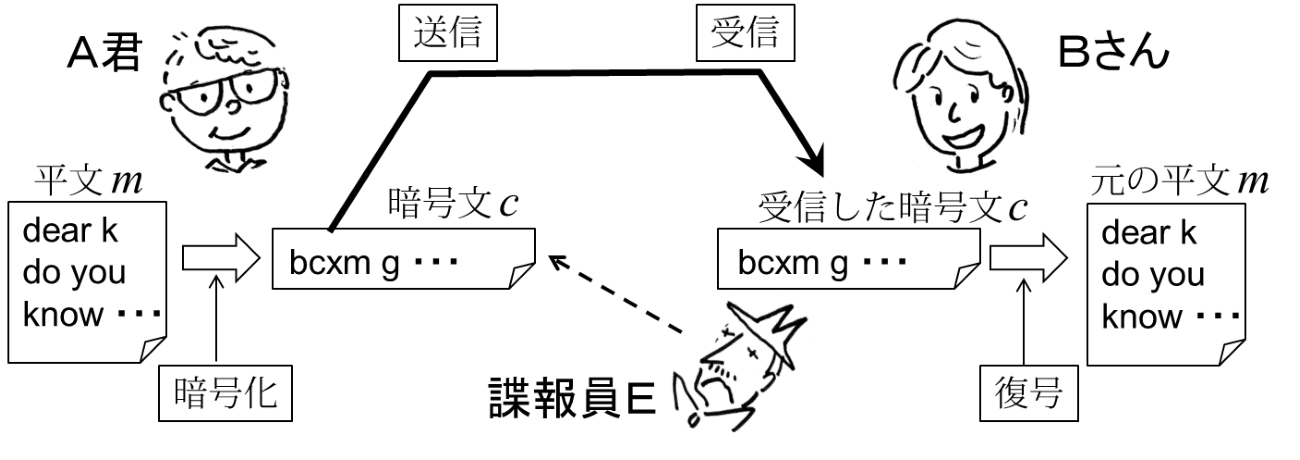
\includegraphics[scale=0.3]{./Figure/elementaryCS-figAliceBob.pdf}
  \end{center}
\end{frame}
\subsection{課題 3}
\begin{frame}[containsverbatim,shrink]
\frametitle{課題 3}
  \begin{itemize}
\item 暗号解読に挑戦
\item \href{https://sites.google.com/presystems.xyz/elementarycs/top}{\beamerbutton{https://sites.google.com/presystems.xyz/elementarycs/top}}に置いてある kaidoku-skeleton.py を参考に暗号解読プログラムを kaidoku.py を作成してください
\item 課題 3 で作成してほしいプログラム
\item 提出は T2Schola からソースコードを提出
  \end{itemize}
\end{frame}
\begin{frame}[containsverbatim,shrink]
\frametitle{暗号解読のヒント}
  \begin{itemize}
\item 意味をなす一般的な文章では文字の出現頻度には偏りがあります
\item たとえば英語では母音 e が最も出現頻度が高い
\item シーザ暗号はこの出現頻度は暗号化しても偏りは変わりません
\item この特徴を利用して何文字移動しているかを予測することができます
\item 各文字 26 個の頻度を計算するために出現回数を要素とする配列をつくる
  \end{itemize}
  \begin{center}
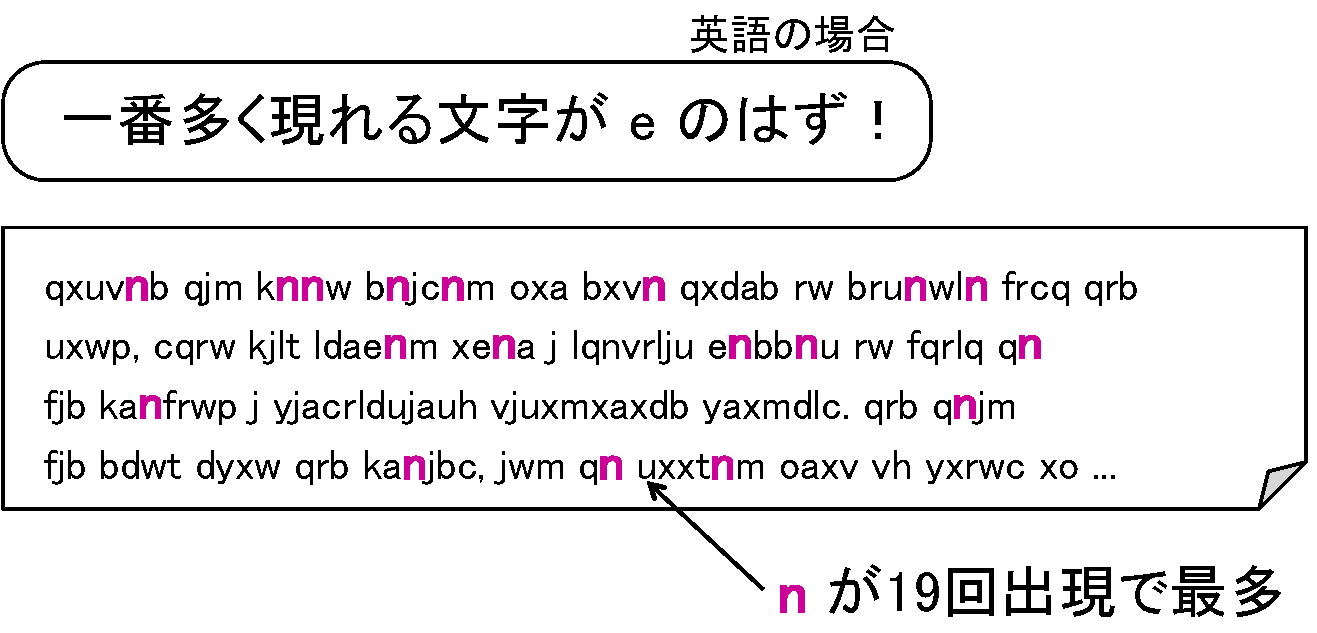
\includegraphics[scale=0.3]{./Figure/elementaryCS-figHintForCryptoanalysis.pdf}
  \end{center}
\end{frame}
\begin{frame}[containsverbatim,shrink]
\frametitle{暗号解読のヒント\textemdash つづき}
  \begin{itemize}
\item 13 番目の文字 n が最多なので 4 番目の文字 e にシフト
\item \(13-4=9\) なので 9 文字シフトしていると推測できる
  \end{itemize}
  \begin{center}
\includegraphics[scale=0.3]{./Figure/elementaryCS-figHindo.pdf}
  \end{center}
\end{frame}
\begin{frame}[containsverbatim,shrink]
\frametitle{暗号解読のヒント\textemdash より高度な方法}
  \begin{itemize}
\item フォーマルには各文字の出現頻度と暗号文での出現頻度の相関\(\phi(i)\)をとります
\item \(\phi(i)=\Sigma_{0\leq c\leq 25}f(c)p(c-i)\), ここで \(f(c)=\frac{n_c}{l_{ct}}\) は暗号文での文字 c の出現頻度,\(p(c-i)\) は一般の出現頻度とする
\item \href{https://sites.google.com/presystems.xyz/elementarycs/top}{\beamerbutton{https://sites.google.com/presystems.xyz/elementarycs/top}}に置いてある 1-gram.txt が出現頻度のファイルです
\item 相関係数 \(\phi(i)\) が
    \begin{itemize}
\item $1$ に近いほど: \(f(c)\) が大きくなれば \(p(c-i)\) も大きくなり相関が強くなる
\item $0$ 近傍: \(f(c)\) と \(p(c-i)\) はあまり相関がない
    \end{itemize}
  \end{itemize}
\end{frame}
